\chapter{Detalles de Implementación}\label{chapter:implementation}

Para la validación de la propuesta planteada a partir del esquema general de definición de los datos de entrada se concibió 
un prototipo de sistema. Este implementa los modelos de generación para el fútbol y el boxeo y permite la interacción
 con los mismos. Para facilitar la interacción se implementó a su vez una interfaz gráfica sencilla. A continuación se presentan 
 detalles generales del sistema, funciones de interés y una presentación de la interfaz creada. Se utilizó \emph{python} como 
 lenguaje de programación.
 
\section{Detalles generales del sistema}

\begin{figure}[!]
    \begin{center}
        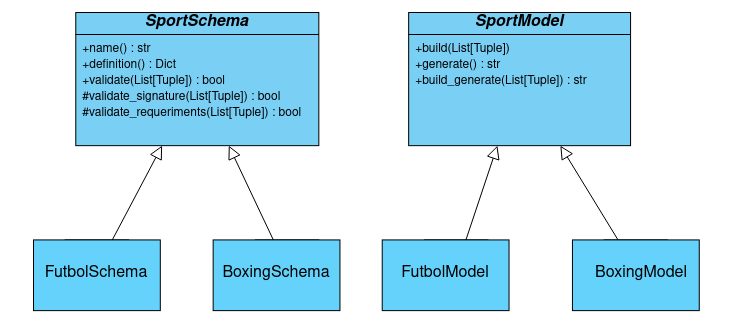
\includegraphics[width=\textwidth]{Graphics/classDef3.png}
    \end{center}
    \caption{Definición de las clases principales}
    \label{fig_classDef}
\end{figure}

Para la representación de los esquemas y de los modelos se crearon dos clases abstractas, \textit{SportSchema} y 
\textit{SportModel}. En la figura (\ref{fig_classDef}) se representan cada una con la signatura principal. 

Los esquemas, con el m\'etodo \emph{validate\_signature}, validan la entrada en cuanto a su signatura, o sea, comprueban que 
su representación en cada uno de los valores se corresponda con la definición. La \textit{definición} (m\'etodo \emph{definition}) 
de un esquema es el conjunto de valores admitidos por cada tipo principal (los tipos principales son los definidos en el 
meta esquema general). A su vez, el método \emph{validate\_requeriments} se utiliza para validar si en el conjunto de entrada
 existe un conjunto minimal de los datos a partir de los cuales es posible la generación de texto. El m\'etodo \emph{name} devuelve 
 un nombre identificativo del esquema, debe ser único. La funcionalidad de \emph{validate} es una conjunción de los otros dos 
 métodos de validación. 




Los modelos para su correcto funcionamiento dependen de un primer llamado al método \emph{build} previo a cualquier 
secuencia de \emph{generate}. El método \emph{build} de los modelos es el que se encarga de procesar la entrada, hacer las 
transformaciones correspondientes de los datos. Durante su ejecución, los modelos completan toda la información 
necesaria para las distintas etapas de generación del texto que se definan. Para esto, se definen estructuras propias de cada 
modelo para representar la información. Con el uso de la información estructurada e interpretada en la construcción del modelo, 
con el método \emph{generate} se generan las distintas piezas textuales que conforman el reporte. El m\'etodo \emph{build\_generate} 
unifica un llamado a \emph{build} seguido de uno a \emph{generate}.

%Los modelos en build tienen que hacer todo el proceso de procesamiento de los datos, llenando tomados
%las variables y estructuras que son necesarias para generar el texto en cada una de las etapas. Luego
%en generate los modelos van en base a la representación interna de los datos, generando el texto de 
%caa una de las piezas comunicativas.

\begin{figure}[!]
    \begin{center}
        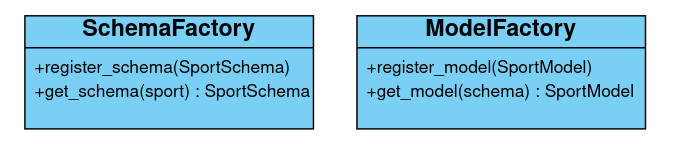
\includegraphics[width=\textwidth]{Graphics/factories.png}
    \end{center}
    \caption{Definición de las clases \emph{Factory}}
    \label{fig_classFactory}
\end{figure}


El flujo principal del programa se encuentra representado en el \textit{Algoritmo Principal} a continuación. Se utilizó el patrón 
\emph{Factory} (de Factoría, en español) para la selección de los modelos y los esquemas (Ver fig\ref{fig_classFactory}). 
Se planteó de esta forma, ya que el prototipo podría adaptarse más fácilmente a nuevos modelos y esquemas sin necesidad de grandes 
cambios en el código. %Las clases \textit{SchemaFactory} y \textit{ModelFactory}

\pagebreak

\begin{verbatim}
Algoritmo principal

  Entrada: knowdlage_tuple:List[Tuple], selected_sport
  Salida : str

    schema = schema_factory.get_schema(selected_sport)
    if not schema.validate(knowdlage_tuple):
        mostrar error
        FIN
    model = model_factory.get_model(schema)
    summary = model.build_generate(knowdlage_tuple)
    return summary

\end{verbatim}



\section{Funciones de realización lingüística}

   El proceso de realización lingüística se lleva a cabo utilizando un conjunto de funciones que permiten la expresión correcta de la información 
en forma de oraciones. Para la representación de los datos los modelos consumen un sistema de plantillas hechas a mano. Un ejemplo de plantilla:

	\begin{center}
		\textit{$<$ portero $>$ atajó un penal a $<$ lanzador $>$ en el minuto $<$ minuto $>$}
	\end{center}

Las expresiones entre $<$ $>$ son las ranuras de las plantillas y se completan utilizando la información procesada de la entrada. Para facilitar la interpretación, 
a la expresión contenida entre $<$ \textit{clave} $>$ se le denominará clave de ranura. Para cada contexto se conciben varias plantillas que permitan realizar la información, 
de forma tal que existan distintas opciones a la hora de expresar una misma idea.

  El proceso de selección y llenado de las plantillas se realiza a través de la función \emph{select\_template} (Algoritmo de selección de plantilla). 
  Esta recibe como parámetros el conjunto de posibles plantillas a emplear, el género a realizar, así como un diccionario de representación de la 
información donde las llaves coinciden con las posibles claves de ranura de las plantillas y los valores son los datos reales. 


  Como el sistema presenta cierto grado de sensibilidad ante la ausencia de algunos datos, es posible que haya plantillas para las que alguna ranura no tenga un 
valor real. La función \emph{\_is\_valid\_template} se utiliza para comprobar esto. El algoritmo selecciona aleatoriamente una plantilla del conjunto, si es válida, 
se selecciona, si no, se descarta y se repite el proceso. Siempre se garantiza que habrá un al menos una plantilla que sea funcional, ya que presentará las ranuras 
correspondientes al subconjunto minimal que admite el sistema en ese contexto. Para comprobar la validez de la plantilla primero 
se detectan las ranuras presentes en esta utilizando la siguiente expresión regular: \textit{(r'$<$ (?P$<$key$>$[a-zA-ZáéíóúÁÉÍÓÚ\_]*) $>$')}.
  
\begin{verbatim}
Algoritmo de selección de plantilla
    
  Entrada: template_group:List[str], data_values:Dict[str,str], 
           genre:Genre.M | Genre.F
  Salida: str
    
    while not valid templat selected:
        template_selected = choice(tempalte_group)
        slots_values = []
        slots = slot_reggex.findall(template_group)
        for slot_value in slots:
            slots_values.append(slot_value)
        if __is_valid_template(slots_values, data_values):
            filled_template = fill_template(template_selected, 
                                slots_values, data_values)
            return disambiguate_template(filled_template, gender)
    return
    
\end{verbatim}   


  El método \emph{fill\_template} sustituye las ranuras de la plantilla por su valor real. Luego se pasa a desambiguar los términos de género. Como el sistema es 
adaptable tanto a la modalidad femenina como masculina de los deportes, es necesario realizar las expresiones en el género correcto. Las ranuras de género están 
presentes en algunas plantillas y tienen esta estructura: \$ clave \$. Estas ranuras se detectan igualmente utilizando una expresión regular similar a la vista 
para las ranuras comunes. El caracter “@” también se utiliza dentro de las plantillas para hacer distinciones de género. Por ejemplo en la frase: \textit{
amb@s se golpearon}, el “@” se sustituye por “a” o por “o” en dependencia del género. Este proceso se produce en la función \emph{disambiguate\_template}.



Otras funciones se utilizan para mejorar el carácter léxico gramatical de las oraciones producidas. La función \emph{ordinal} transforma expresiones numéricas 
en su expresión ordinal (primer, segundo,  tercer, ..., vigésimo). La función numeral transforma un valor numérico en su expresión léxica (uno, dos, tres). Esta 
abarca los números desde el 1 al 20 y los múltiplos de 10 hasta 100. Una vez que todas las transformaciones sobre las plantillas han sido realizadas, la función 
\emph{sentence\_lexical\_realization}, se utiliza para eliminar posibles errores, como espacios dobles, repetición de artículos (“el EL”), o corrige errores 
transformando expresiones como “de el” en su forma correcta “del”.



\section{Interfaz gráfica}

Para poder interactuar más fácil con la propuesta, se proporcionó una interfaz gráfica. Esta interfaz es sencilla
y se concibió utilizando el \emph{framework} de \textit{python streamlit}. Se da la opción a los usuarios de aportar
 datos en forma de archivos, ya sea a partir de definir la ruta local o cargando directamente el archivo.

 Para permitir  esta interacción se concibió una estructura intermedia para poder representar las tuplas 
de entrada en archivos \textit{.json} (ver fig\ref{fig_jsonexample}). Cada tupla se representa con las llaves: “1”, “2”,“3”,“4”
donde cada valor correspondiente representa el valor de la tupla en esa posición. Si no se proporciona uno de los 
valores, esa posición se considera vacía.

    \begin{figure}[!]
        \begin{center}
            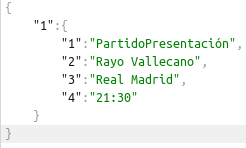
\includegraphics[scale=0.6]{Graphics/jsonexample.png}
        \end{center}
        \caption{Ejemplo de representación intermedia de una tupla de entrada en formato \textit{json}}
        \label{fig_jsonexample}
    \end{figure}

 Desde la primera interfaz se puede interactuar con el conjunto de datos de prueba que se concibieron
junto a la propuesta. Para ello hay que seleccionar el deporte deseado y uno entre los eventos de prueba.
El sistema mostrará el texto producido en pantalla, luego de presionar el botón “generar”.



\begin{figure}[!]
    \begin{center}
        
\includegraphics[width=\textwidth]{Graphics/GRED.png}
    \end{center}
    \caption{Interfaz del sistema}
    \label{fig_interfaz}
\end{figure}
